\chapter{Data Processing and and Loading}
This chapter will discuss how to prepare the users training data to be in the correct format to feed into the convolutional neural network. PyTorch allows for the data to be fed in a variety of different ways. Their CNN tutorial online uses small images that are labelled using a csv to flag where certain features in the training images are. Our network differs from this and assumes the user has two folders, one with RGB rasters and another with matching ground truth images that are rasters with max and min values corresponding to where the items of interest are in the similarly named RGB raster. 

\begin{figure}[htbp]
    \centering
    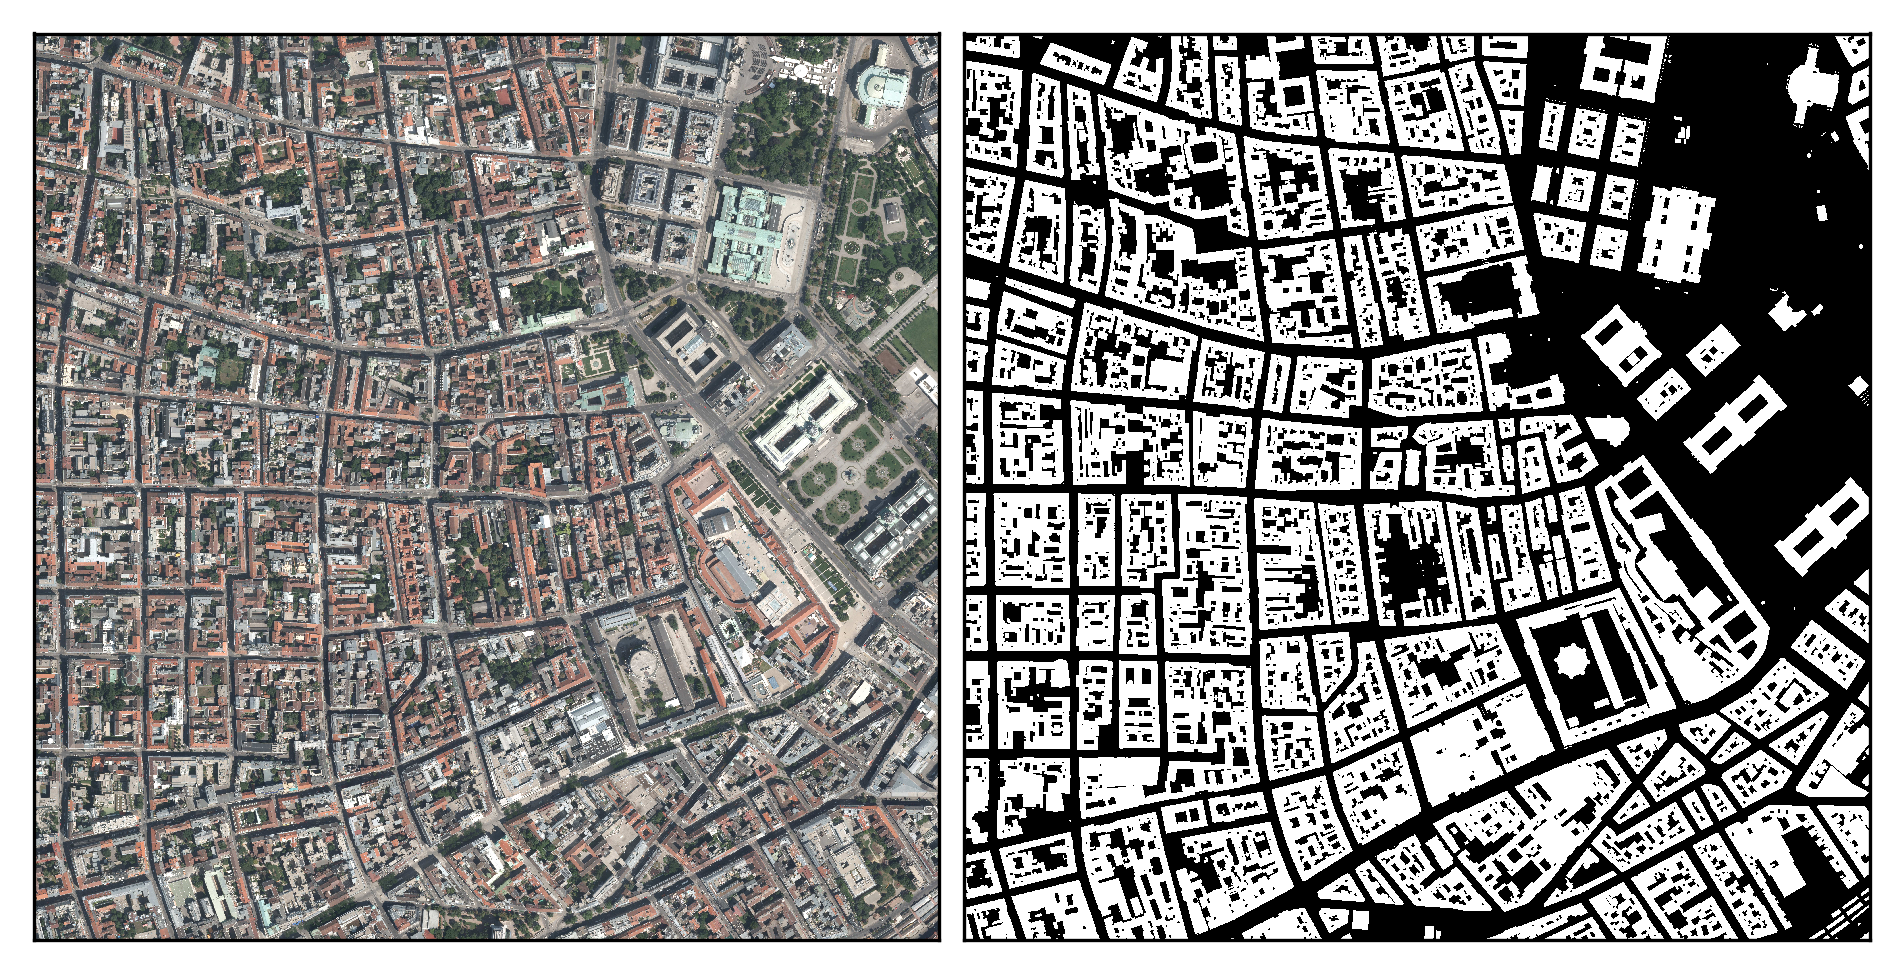
\includegraphics[width=1\textwidth]{\dir/figs/example_data.png}
    \caption[Side by Side comparison of RGB image and ground truth]{The grid on the left shows the original binary classification, where white shows the class of interest and the black shows nothing. On the right, the upper grid shows white where the original image showed white. On the right the lower grid shows white where the original grid showed black.}
    \label{fig.example_data}
\end{figure}


\section{Pre-Processing the Data}
In order for the image data to work within PyTorch it needs to be in the Python Imaging Library Format (PIL) format. The training and test dataset used for the creating of the workflow were in .tif format and so no conversion was needed. If the data type the user intended to use was not in the PIL format, a conversion would be necessary.
\par
The training data first needs to be split into training, validation and testing datasets. During training the model will not touch the test dataset, this is in order to test the overall accuracy of the network. I wrote a custom script in order to do this, that uses PyTorch's subset sampler function.
\section{Transform the Data}
For a user wanting to load and train a network they first need to prepare their data so that it is in the right format to be read by the network. In remote sensing, a user may commonly have an image of 30,000x30,000 pixels if they have a 10x10km tile at ~30cm resolution. This needs to be transformed and reduced in size to train a network. The networks would not be trained well if just one image was fed in, especially at the extreme size of 30,000x30,000 pixels. The first step of the process is to transform and crop this data so that only a small section of the image is being fed into the network. I have created a class for clipping and tiling the images that then can be fed into the CNN (Listing \ref{lst.transform}).
Transforms on the data need to be performed on both the image layer and the binary mask in tandem. It is necessary to perform the transform in order to reduce the spatial dimensions of the input volume and synthesis more training samples. By taking a 128x128 pixel random crop, from each 5000x5000 pixel training sample, each iteration, the number of training samples will increase. A custom transform class script was written to ensure that these transformed were mirrored and the two layers of information remained paired and not distorted (Listing \ref{lst.transform}). If the transformation is not performed in tandem then when the network compares the predicted output to the ground truth output, the two images will not aligned.
The arguments for the transform class are lists of all the users image and associated and binary mask files. The user can remove the comment at Listing \ref{lst.transform} line 16-19 if their training data is not all of the same dimensions. The class then proceeds to crop, horizontally flip, vertically flip, and eventually transform the data arrays into PyTorch tensors that can be fed into PyTorch's neural network data loader class. 
\par 
 \begin{lstlisting}[language=Python, caption = {Transform Class for buidling the dataset class, which can be input into the dataloader class, which in turn is iterated over in the CNN.}, label={lst.transform},float,floatplacement=htbp]
class BuildingsDataset(Dataset):
    """INRIA buildings dataset"""
    def __init__(self,images_dir,gt_dir,train=True):
        """
        Args:
        images_dir = path to the satellite images
        gt_dir = path to the binary mask
        """
        self.image_paths = images_dir
        self.target_paths = gt_dir
        self.train=train
        
    def transform(self, image, mask):
        # Resize
#         resize = transforms.Resize(size=(5000, 5000))
#         image = resize(image)
#         mask = resize(mask)

        # Random crop
        i, j, h, w = transforms.RandomCrop.get_params(
            image, output_size=(256, 256))
        image = TF.crop(image, i, j, h, w)
        mask = TF.crop(mask, i, j, h, w)
        
        # Random horizontal flipping
        if random.random() > 0.5:
            image = TF.hflip(image)
            mask = TF.hflip(mask)
            
        # Random vertical flipping
        if random.random() > 0.5:
            image = TF.vflip(image)
            mask = TF.vflip(mask)
            
        # Transform to tensor
        image = TF.to_tensor(image)
        mask = TF.to_tensor(mask)
        mask = torch.cat([(mask==0).float(),(mask==1).float()],dim=0)
        return image, mask
        
    def __getitem__(self, index):
        image = Image.open(self.image_paths[index])
        mask = Image.open(self.target_paths[index])
        x, y = self.transform(image, mask)
        return x, y
        
    def __len__(self):
        return len(self.image_paths)
\end{lstlisting}
There is an additional transformation that is applied to the mask. The binary mask comes as one layer where the minimum value corresponds to what is not of interest and the max value corresponds to where there is something of interest (Listing \ref{lst.transform} line 39). The transform splits this single layer into two layers. In the first layer, where the value was minimum it now shows as max and the opposite is the case for the second layer (Figure \ref{fig.binary_mask}) . This is so that when a class probability is determined by the network this can then predict which layer the pixel is most likely to belong to. In essence this process has transformed the data into two classes rather than just one.
\begin{figure}[htbp]
    \centering
    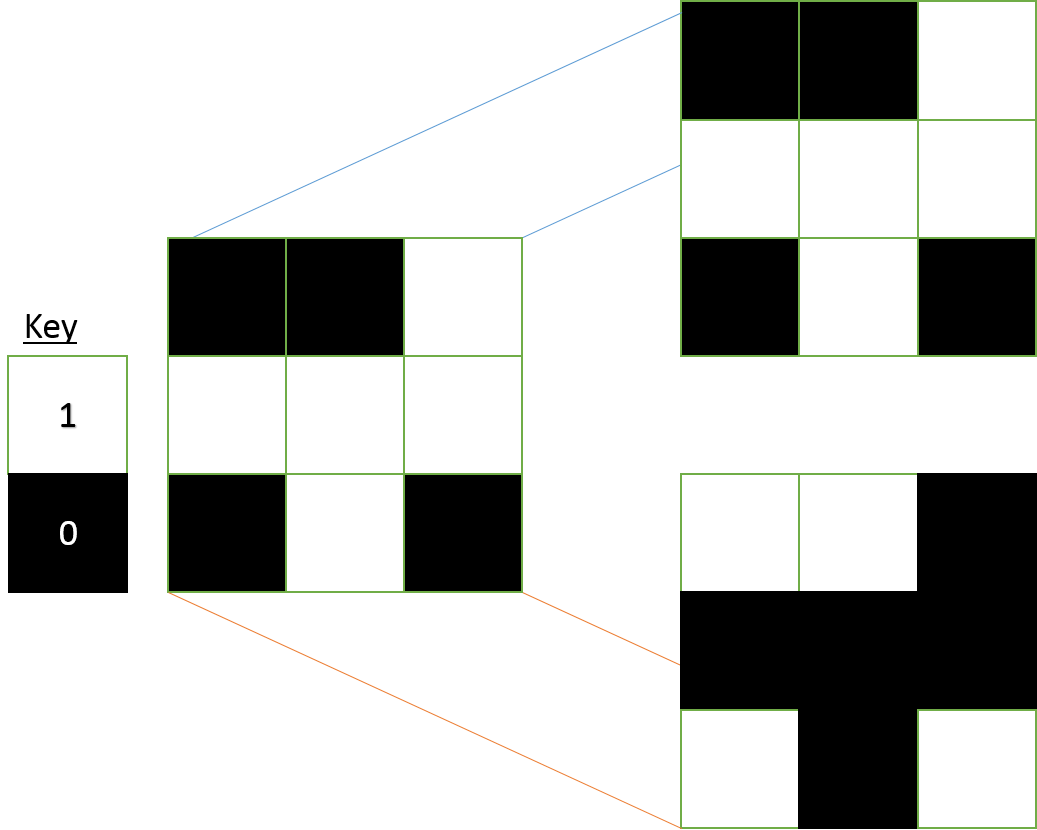
\includegraphics[width=0.5\textwidth]{\dir/figs/binary_mask.png}
    \caption[Binary Mask]{The grid on the left shows the original binary classification, where white shows the class of interest and the black shows nothing. On the right, the upper grid shows white where the original image showed white. On the right the lower grid shows white where the original grid showed black.}
    \label{fig.binary_mask}
\end{figure}
The transform function outputs an array with two item, where the first item is the image as a tensor and the second item is the associated binary mask as a tensor. This datatype is then ready to be loaded directly into the neural network.
\section{Load the Data}
PyTorch has a in-built dataloader class that is used to batch and load the data. It can even be used to load the data using GPU if the user had access to one. The data needs to be prepared in a certain way in order to be loaded through this class. The transform class prepares the data into this specific format so it can be bulk loaded into the network. The dataloader then batches, shuffles and loads the data, either in parallel or not, into the neural network for training. Figure \ref{fig.dataloader} shows how the data looks as it is being fed into the CNN. There is a randomly cropped RGB image with an associated binary mask, which is made up of two layers, the first layer being displayed as 1 where the class is, the second showing 1 where the class is not. 
\begin{figure}[H]
    \centering
    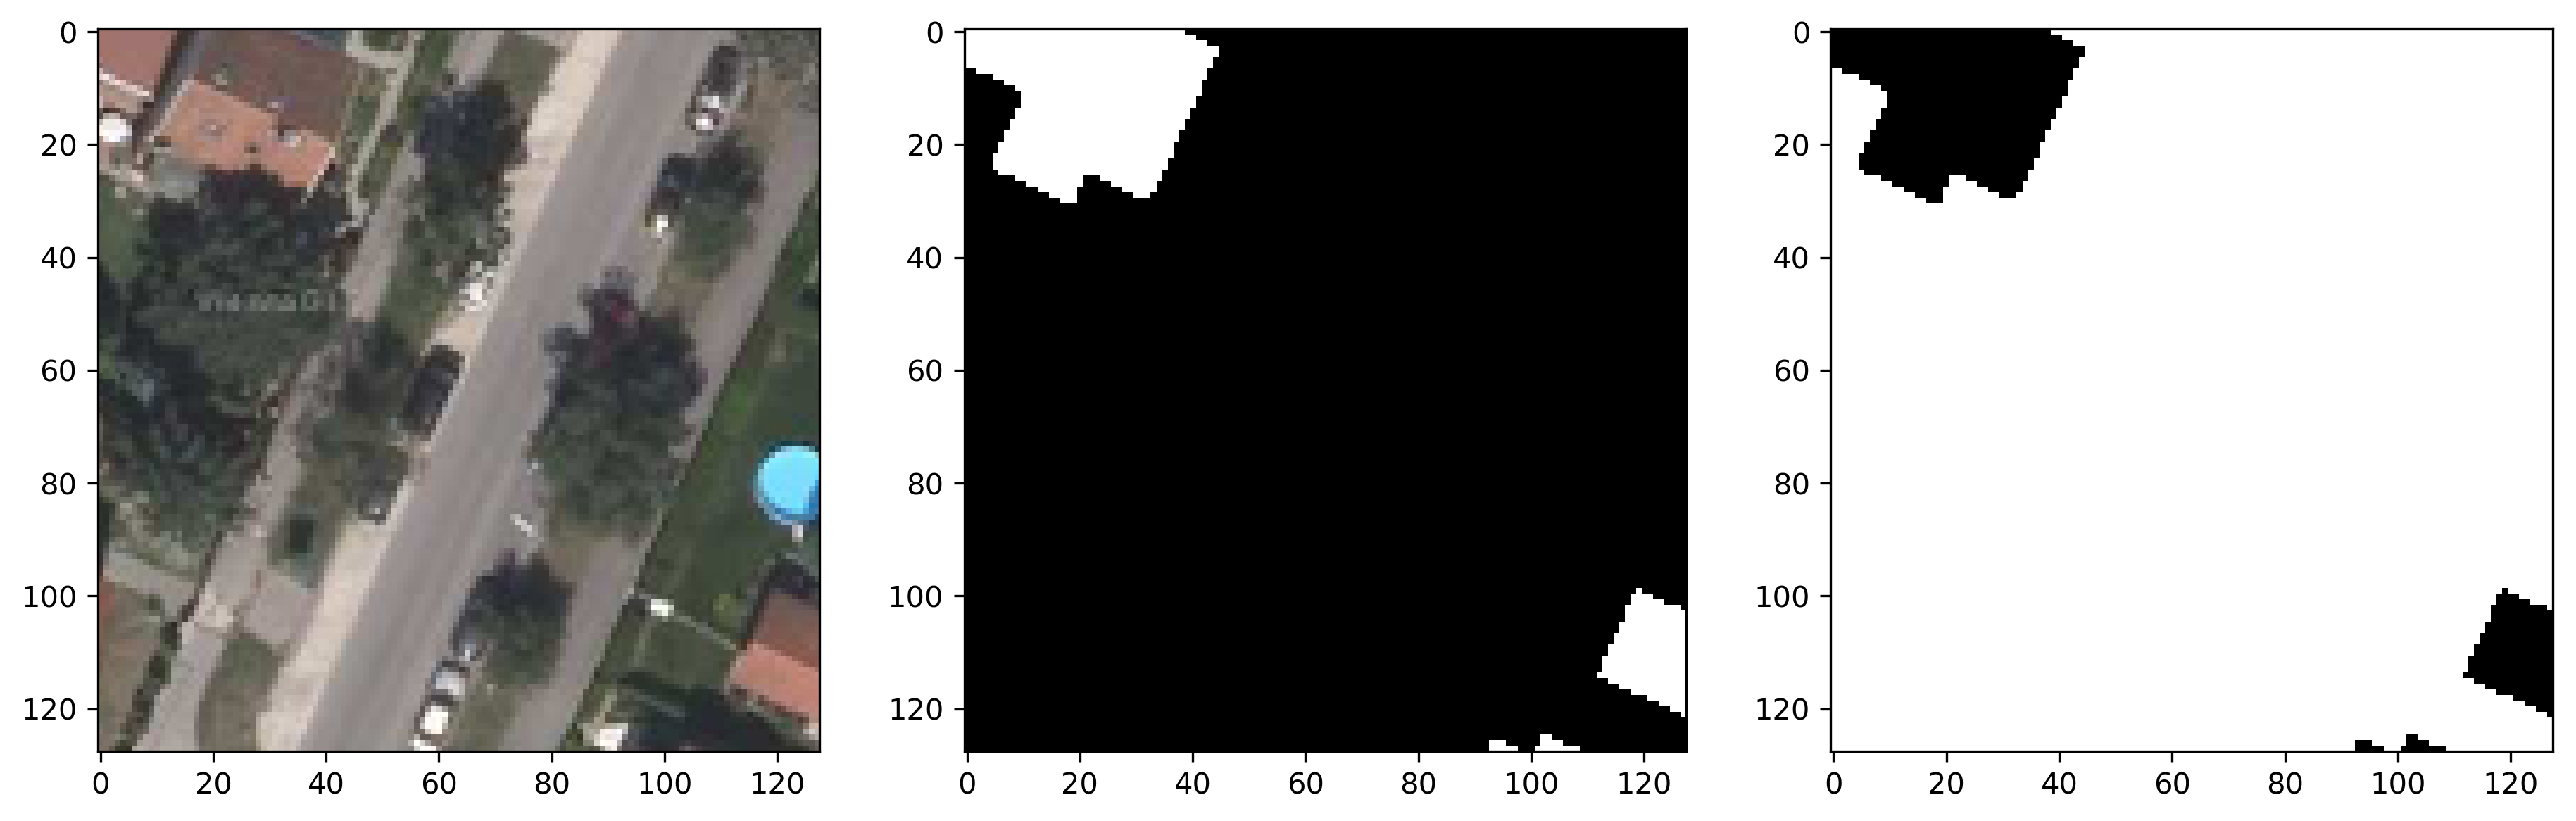
\includegraphics[width=1\textwidth]{\dir/figs/example_dataloader.png}
    \caption[Example of how the dataloader handles the data]{Example of how the dataloader handles the data. This image shows a random 128x128 crop from a random tile within the dataset. The dataloader constructs these paired images into a stack that can be defined by the user and optimised to reduce processing times. On the left is the RGB image, the middle shows as positive where there are buildings and the left shows as positive where buildings are not. The two images on the right are taken from the ground truth dataset.}
    \label{fig.dataloader}
\end{figure}